\documentclass[11pt, titlepage]{article}
\usepackage{amsmath,amsthm,amssymb}
\usepackage{hyperref, pgf, tikz}
\usepackage{fancyhdr}
\usetikzlibrary{arrows}
\usepackage[margin=1.25in]{geometry}
\usepackage{graphicx}                     
\pagestyle{fancy}
\usepackage{array}
\usepackage{indentfirst}
%\usepackage{wrapfig}

\lhead{Lab \#6}
\rhead{\thepage}
\cfoot{}

\title{Introduction to the Microwave Optics System and Reflection \\ \ \\ \large Lab \#6}
\author{Name: Avery Karlin \\ Partner: Dalton Wu}
\date{}
\begin{document}

\maketitle

\begin{center}
\LARGE Introduction to the Microwave Optics System and Reflection
\end{center}

\section*{Objective}
The objective of the lab is to practice using the microwave optics system, measure the relationship between distance and microwave strength, and test the law of reflection.

\section*{Introduction}
Electromagnetic radiation is perpendicular transverse waves of magnetic and electric fields, all moving at the speed of light ($3 * 10^8$ m/s), ranging in type based on frequency and energy, with higher frequency meaning higher energy. The most high energy is gamma radiation, produced by nuclear reactions only, unlike all other forms which are produced by electronic movement. The next longest is x-rays, used in medical testing, followed by ultraviolet, then visible light (the only type humans can see), followed by infrared (used for night vision, based on black body radiation), then microwave radiation, and finally radio waves (used for all electronic communication signals).

Electromagnetic radiation can be polarized by a polarizer, only allowing waves of a specific orientation through, such that perpendicular polarizers block all waves as a result. Microwave strength is inversely proportional to the square of the distance, such that it decreases exponentially. In addition, the law of reflection states that if the radiation is reflected, the angle of incidence is equal to the angle of reflection, such that the microwave radiation picked up is greatest at that angle from it.

\section*{Procedures and Results}

First, the transmitter and receiver are hooked onto the fixed arm, which is then fixed on the goniometer sliding measuring bar. After, the receiver must be set to 30x and then calibrated by the variable sensitivity dial, until the reading is 1 for 0.4 distance between the transmitter and receiver. It is then measured as the distance between them increases by 10 cm intervals until there is 1 meter between, recording the reading. 

A reflector, parallel to the axis between the transmitter and receiver, has a reflector then moved closer to it to determine the change in readings, increasing as the reflector moves closer, due to the waves moving away from the axis reflecting back towards it.

After, the hand screw connecting the receiver to the fixed arm is loosened, such that it can be rotated, receiving from the same direction, but in different orientations, watching the change in reading on it. It is thus seen that when the orientations are perpendicular to each other, rather than parallel or anti-parallel, the readings on the receiver is 0, at the maximum when parallel or anti-parallel.

Next, the receiver is rotated, such that the angle between it and the original position is recorded for intervals of 10 degrees, measuring the meter reading, such that it starts at 1 for $0^o$. Finally, it is set up similarly, with a reflector attached in the center, such that the angle of incidence is modified by rotating the reflector, then rotating the receiver, such that the angle of reflection to the receiver changes, finding the angle where the reading is greatest.

\begin{figure}[h]
\centering
\hspace*{0cm}
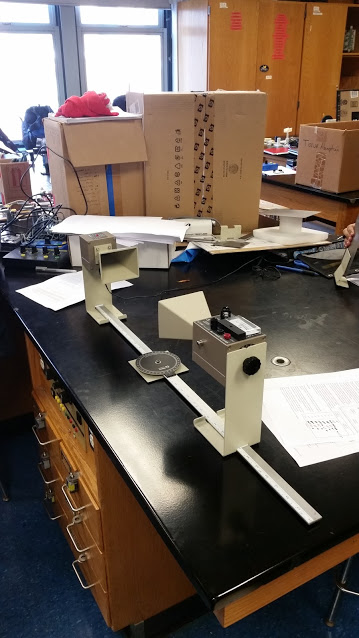
\includegraphics[scale=1]{lab61.jpg}
\vspace*{0cm}
\end{figure}

\begin{figure}[h]
\centering
\hspace*{0cm}
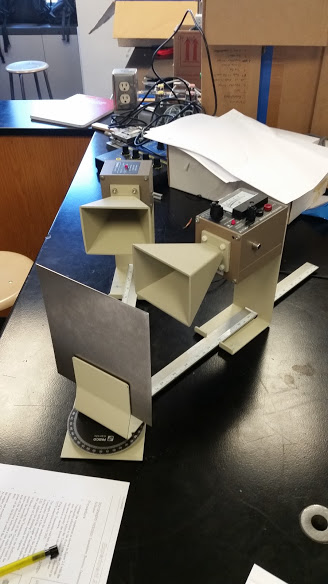
\includegraphics[scale=1]{lab62.jpg}
\vspace*{0cm}
\end{figure}

\underline{Wave Strength vs Distance:}
\begin{center}
\begin{tabular}
{|m{9em}|m{18em}|}
\hline
Distance (m) & Microwave Radiation Strength (M) \\
\hline
0.4 & 1\\
\hline
0.5 & 0.58\\
\hline
0.6 & 0.38\\
\hline
0.7 & 0.3\\
\hline
0.8 & 0.18\\
\hline
0.9 & 0.08\\
\hline
1 & 0.04\\
\hline
\end{tabular}
\end{center}

\underline{Wave Strength vs Angle:}
\begin{center}
\begin{tabular}
{|m{9em}|m{18em}|}
\hline
Angles $(^o)$ & Microwave Radiation Strength (M) \\
\hline
0 & 1\\
\hline
10 & 0.52\\
\hline
20 & 0.36\\
\hline
30 & 0.04\\
\hline
40 & 0.02\\
\hline
50 & 0.01\\
\hline
60 & 0\\
\hline
70 & 0\\
\hline
80 & 0\\
\hline
90 & 0\\
\hline
\end{tabular}
\end{center}

\underline{Angle of Incidence vs Angle of Reflection:}
\begin{center}
\begin{tabular}
{|m{12em}|m{12em}|}
\hline
Angle of Incidence $(^o)$ & Angle of Reflection $(^o)$ \\
\hline
10 & 10\\
\hline
20 & 20\\
\hline
30 & 27.5\\
\hline
40 & 35\\
\hline
50 & 45\\
\hline
60 & 65\\
\hline
70 & 60\\
\hline
80 & 70\\
\hline
90 & 70\\
\hline
\end{tabular}
\end{center}

\section*{Discussion}
Sample calculations for the non-measured data are as shown using the formulas found above:

$$\text{Microwave Radiation Strength * Distance (0.4 m Distance)} = R * M = 0.4 * 1 = 0.4 m$$
$$\text{Microwave Radiation Strength * Distance$^2$ (0.4 m Distance)} = R^2 * M = 0.4^2 * 1 = 0.16 m^2$$

\underline{Wave Strength vs Distance:}
\begin{center}
\begin{tabular}
{|m{15em}|m{15em}|}
\hline
Microwave Radiation Strength * Distance (m) & Microwave Radiation Strength * Distance$^2$ $(m^2)$ \\
\hline
0.4 & 0.16\\
\hline
0.29 & 0.145\\
\hline
0.228 & 0.137\\
\hline
0.21 & 0.147\\
\hline
0.144 & 0.115\\
\hline
0.072 & 0.065\\
\hline
1 & 0.04\\
\hline
\end{tabular}
\end{center}

The values for the microwave strength reading multiplied by the square of the distance are fairly similar, with slightly varying readings at the extremes of the distance, most likely due to the lack of specificity of the receiver readings at those points. In addition, due to being less accurate at further distances, this could be due to waves escaping in the space between. On the other hand, it is apparent from the readings that as the distance increases, the meter reading decreases exponentially. As a result, since the electric field is inversely proportional to the distance, while the wave intensity is inversely proportional to the square of the distance, the meter signifies the wave intensity, rather than the electric field.

It is apparent that as the reflector is moved closer to the area between the transmitter and the receiver, the readings increased, most likely due to rays that would have gone outside of the space between the two, away from the receiver, reflected back toward the receiver, catching more as it is moved closer.

When the receiver is rotated, such that the polarity/direction of the horn is different from that of the transmitter, the reading decreases until it is at 0 when they are perpendicular to each other, such that the wave is shown to be planar, moving perpendicular to the direction of propagation, rather than spherical, in all directions, such that polarizing can cancel out the entire wave.

For the rotation of the receiver without a reflector, the reading decreases the larger the rotation is as expected, due to fewer of the waves being able to enter the receiver, decreasing exponentially, due to the higher amount of waves moving straight, with only a few diverging, far more likely to only diverge slightly.

While the readings of the receiver with a reflector partially followed the law of reflections (angle of incidence is equal to the angle of reflection), such that the maximum angle of reflection was close to the angle of incidence, only for the lower angles was it precisely equal. This is due to the receiver detecting both the reflected wave and the wave from the transmitter, due to not all waves hitting the reflector at the same angle, and some waves bypassing the reflector, such that it will change the results. At other angles, there were still readings, if not lower, due to not all rays hitting at the same angle, due to the lack of specificity of the transmitter, such that it was reflected at different angles, which would not be the case with perfect plane waves, in which case they would all hit at the same angle, and thus it would be precise for all.

\section*{Conclusion}
Electromagnetic radiation behaves as a plane wave, where the intensity of the wave is inversely proportional to the distance squared from the source. It is reflected by the law of reflections such that the angle of incidence against the reflector is equal to the angle of reflection.


\end{document}
